\documentclass[]{article}
\usepackage[a4paper,top=3cm,bottom=2.5cm,left=2.5cm,
            right=2cm,marginparwidth=1.75cm,
            headheight=5pt]{geometry}
\usepackage[T5]{fontenc}
\usepackage[utf8]{inputenc}
\usepackage[document]{}
\usepackage[english]{babel}
\usepackage[unicode]{hyperref}
\usepackage{amsmath}
\usepackage{setspace}
\usepackage{graphicx}
\usepackage{caption}
\usepackage{subcaption}
\usepackage{tcolorbox}
\usepackage{listings}
\usepackage{hyperref}
\usepackage{xcolor}
\usepackage{longtable}
\usepackage{titlesec}
\usepackage{floatrow}
\usepackage[nottoc]{tocbibind}
\usepackage{mdframed}
\usepackage{amsmath}
\usepackage{amssymb}
\usepackage{tgbonum}
\usepackage{type1cm}
\usepackage{indentfirst}
\usepackage{lettrine}
\usepackage{colortbl}
\usepackage{fancyhdr}
\usepackage{wrapfig}
\usepackage{lastpage}
\usepackage{url}
\addto\captionsenglish{
  \renewcommand{\contentsname}{Table of Contents}%
  \renewcommand{\listfigurename}{Danh sách ảnh}%
  \renewcommand{\listtablename}{Danh sách bảng}%
  \renewcommand{\figurename}{Figure}
  \renewcommand{\tablename}{Table}
}
\pagestyle{fancy}
\fancyhf{}
\rhead{Intro to Machine Learning}
\lhead{\color{cyan}Google Data Analytics by Coursera}
\lfoot{Page \thepage /\pageref{LastPage}}
\renewcommand{\footrulewidth}{0.4pt}
\setlength{\parindent}{1.5em}
\setlength{\parskip}{1cm}
\renewcommand{\baselinestretch}{1.5}
\newmdenv[linecolor=black,skipabove=\topsep,skipbelow=\topsep,
leftmargin=2.5cm,rightmargin=2.5cm,
innerleftmargin=5cm,innerrightmargin=5cm]{mybox}
\usepackage{multicol}
\usepackage{indentfirst}
\usepackage{color}
\usepackage{tikz}
\graphicspath{{Figures/}} 
\usepackage{lipsum}
\usetikzlibrary{calc}
\setlength{\columnseprule}{2pt}
\def\columnseprulecolor{\color{black}}
\def\maru#1{\textcircled{\scriptsize#1}}

\usepackage[backend=biber, style=numeric]{biblatex}
\addbibresource{refs.bib} % Tải tệp references.bib
\defbibheading{mybibintoc}{\section{Tài liệu tham khảo}}


\begin{document}

% Bìa trang
\begin{titlepage}
  \begin{tikzpicture}[remember picture,overlay,inner sep=0,outer sep=0]
    \draw[blue!70!black,line width=4pt] ([xshift=-1.5cm,yshift=-2cm]current page.north east) coordinate (A)--([xshift=2cm,yshift=-2cm]current page.north west) coordinate(B)--([xshift=2cm,yshift=2cm]current page.south west) coordinate (C)--([xshift=-1.5cm,yshift=2cm]current page.south east) coordinate(D)--cycle;

    \draw ([yshift=0.5cm,xshift=-0.5cm]A)-- ([yshift=0.5cm,xshift=0.5cm]B)--
    ([yshift=-0.5cm,xshift=0.5cm]B) --([yshift=-0.5cm,xshift=-0.5cm]B)--([yshift=0.5cm,xshift=-0.5cm]C)--([yshift=0.5cm,xshift=0.5cm]C)--([yshift=-0.5cm,xshift=0.5cm]C)-- ([yshift=-0.5cm,xshift=-0.5cm]D)--([yshift=0.5cm,xshift=-0.5cm]D)--([yshift=0.5cm,xshift=0.5cm]D)--([yshift=-0.5cm,xshift=0.5cm]A)--([yshift=-0.5cm,xshift=-0.5cm]A)--([yshift=0.5cm,xshift=-0.5cm]A);


    \draw ([yshift=-0.3cm,xshift=0.3cm]A)-- ([yshift=-0.3cm,xshift=-0.3cm]B)--
    ([yshift=0.3cm,xshift=-0.3cm]B) --([yshift=0.3cm,xshift=0.3cm]B)--([yshift=-0.3cm,xshift=0.3cm]C)--([yshift=-0.3cm,xshift=-0.3cm]C)--([yshift=0.3cm,xshift=-0.3cm]C)-- ([yshift=0.3cm,xshift=0.3cm]D)--([yshift=-0.3cm,xshift=0.3cm]D)--([yshift=-0.3cm,xshift=-0.3cm]D)--([yshift=0.3cm,xshift=-0.3cm]A)--([yshift=0.3cm,xshift=0.3cm]A)--([yshift=-0.3cm,xshift=0.3cm]A);

  \end{tikzpicture}
  \newcommand{\HRule}{\rule{\linewidth}{0.5mm}}
  \center

  \textsc{\Large UNIVERSITY OF SCIENCE}\\[0.5cm]
  \textsc{\Large FACULTY OF INFORMATION TECHNOLOGY}\\[1cm]
  
\includegraphics[width=0.3\textwidth]{logo/KHTN.jpg}\\[1cm]

  \HRule \\[0.4cm]
  {\huge \bfseries GOOGLE DATA ANALYTICS} \\[0.4cm]
  {\large COURSERA}\\[0.1cm]
  \HRule \\[1.5cm]

  \centerline{\Large{\textbf{Triệu Nhật Minh — 21127112 — 21KHMT2}}}
  \vspace{2.5cm}
  \centerline{\large{\textit{Giảng viên hướng dẫn}}}
  \vspace{0.25cm}
  \centerline{\large{Bùi Duy Đăng}}
  \centerline{\large{Phạm Trọng Nghĩa}}
  \centerline{\large{Nguyễn Ngọc Đức}}
  \vspace{3cm}
  \centerline{\today}


  \vfill % Wipe blank space of the page.
\end{titlepage}

% Mục lục tự động
\setlength{\parskip}{.7em}
\tableofcontents
\newpage

% Table of Figures & Tables
\setlength{\parskip}{.5em}
%\listoffigures
%\listoftables
\newpage

% Bắt đầu nội dung

\section{Certificate}
\subsection{Professional Certificate: Google Data Analytics by Coursera}
\begin{figure}[!h]
  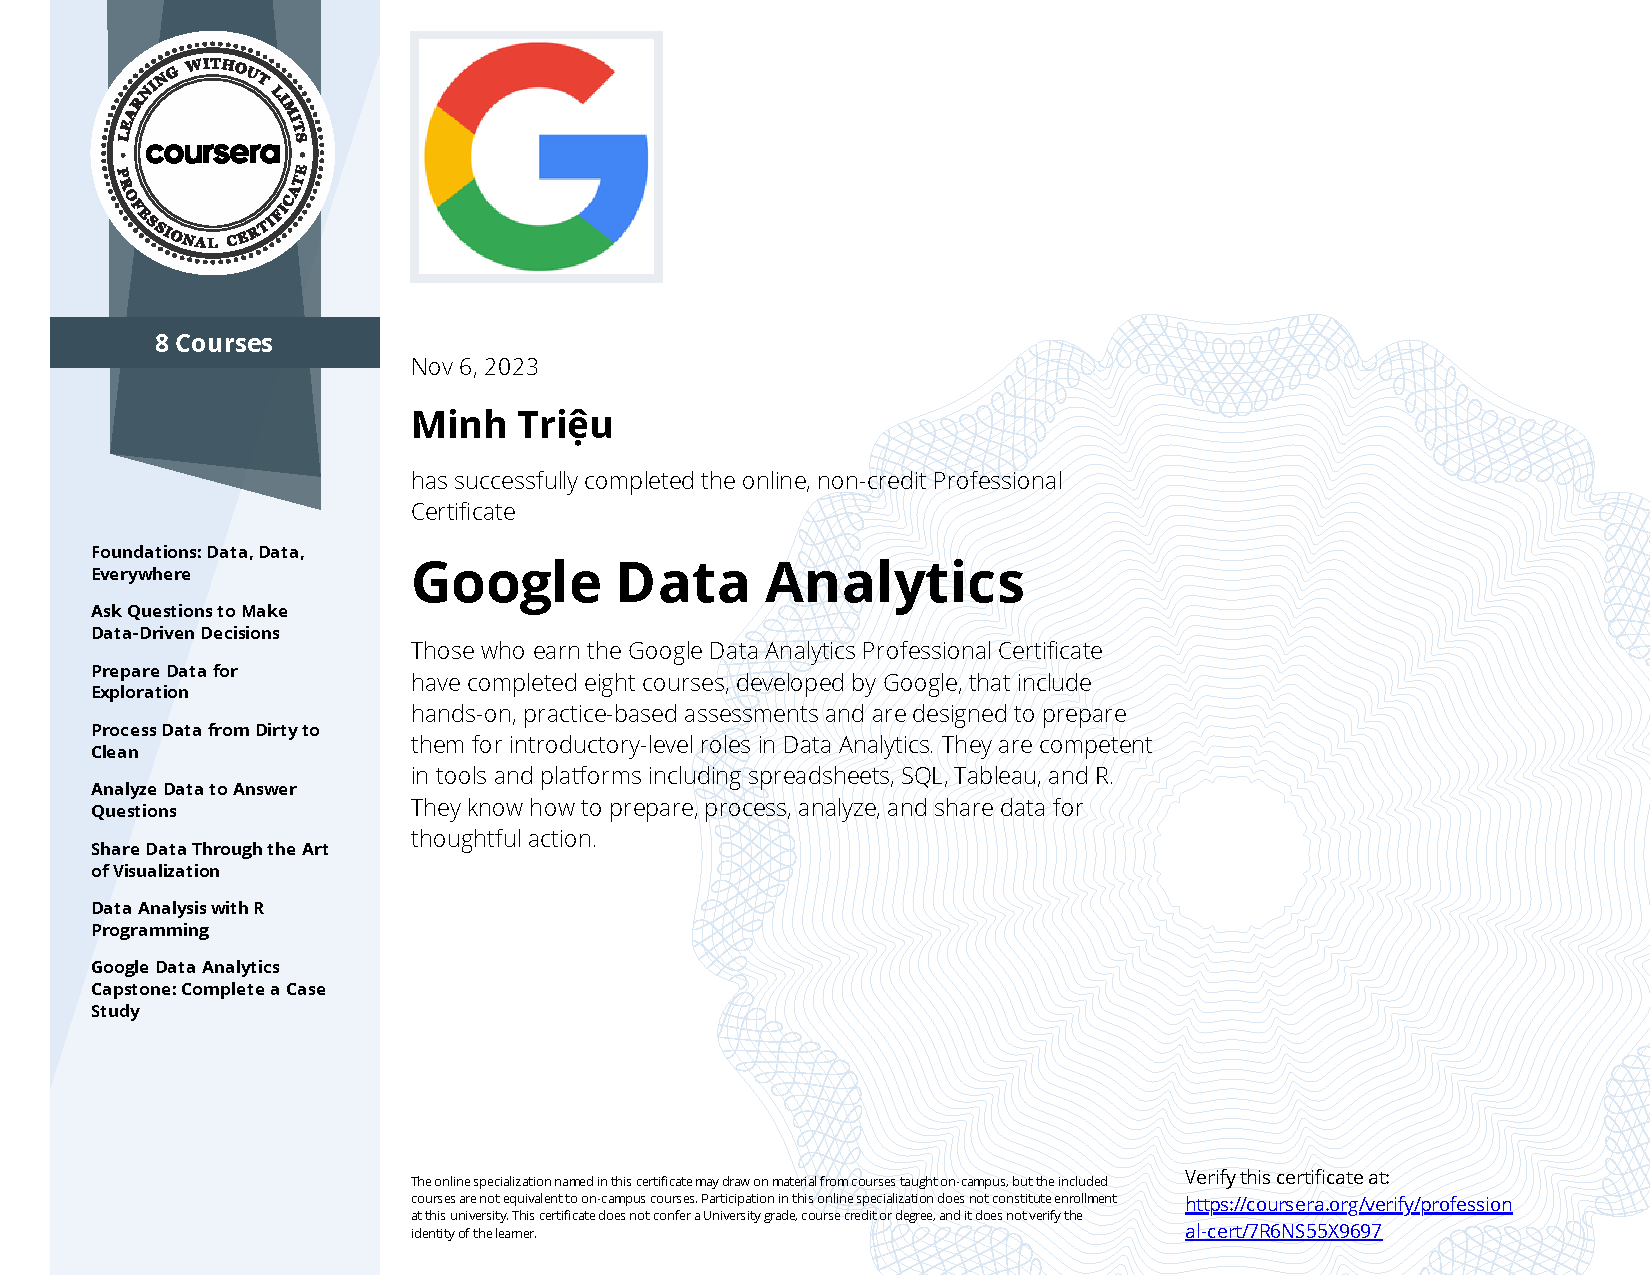
\includegraphics[width=0.8\textwidth]{certs/7R6NS55X9697.pdf}
  \caption{\href{https://www.coursera.org/account/accomplishments/specialization/certificate/7R6NS55X9697}{Verification}}
\end{figure}

\subsection{Enrollment date (8 courses)}
\begin{enumerate}
  \item \href{https://www.coursera.org/account/accomplishments/certificate/S9CWWMGFJAMM}{Foundations: Data, Data, Everywhere - 22nd October 2023}
  \item \href{https://www.coursera.org/account/accomplishments/certificate/ZA7TH6KEEEPB}{Ask Questions to Make Data-Driven Decisions - 24th October 2023}
  \item \href{https://www.coursera.org/account/accomplishments/certificate/B7PZ38G3U9XR}{Prepare Data for Exploration - 27th October 2023}
  \item \href{https://www.coursera.org/account/accomplishments/certificate/DYHS63889XUN}{Process Data from Dirty to Clean - 29th October 2023}
  \item \href{https://www.coursera.org/account/accomplishments/certificate/6478SYGTR4HF}{Analyze Data to Answer Questions - 5th November 2023}
  \item \href{https://www.coursera.org/account/accomplishments/certificate/8JULNPUM3GLC}{Share Data Through the Art of Visualization - 6th November 2023}
  \item \href{https://www.coursera.org/account/accomplishments/certificate/JPHDNMYYDJZ9}{Data Analysis with R Programming - 6th November 2023}
  \item \href{https://www.coursera.org/account/accomplishments/certificate/7TN58662AD9X}{Google Data Analytics Capstone: Complete a Case Study - 6th November 2023}
\end{enumerate}
Completion date of each course: On certificate verification link.

\section{Course 1: Foundations: Data, Data, Everywhere}
\begin{itemize}
  \item The introductory part of the course was a fascinating journey into the world of data analytics. I gained valuable insights into the role and skills of a data analyst, and how data influences decision-making processes in various contexts.
  \item The second part of the course allowed me to delve deeper into the life cycle of data and the process of data analysis. I learned about the stages of data collection, processing, analysis, and communication, and the tools and techniques used at each stage. I also honed my analytical thinking skills and learned to ask insightful questions.
  \item In the third part of the course, I mastered the basics of spreadsheets, query languages, and data visualization tools. I learned to organize, manipulate, and analyze data using spreadsheets, perform calculations using formulas and functions, query data from databases using SQL, and create interactive dashboards and charts using Tableau.
  \item In the fourth part of the course, I explored the diverse range of businesses and industries that leverage data analytics, and the career opportunities available for data analysts. I also prepared for the Google Data Analytics Certificate and learned how to showcase my skills and portfolio.
  \item Finally, I successfully completed the Course Challenge, which tested my understanding of the main concepts and terms covered in the course. I applied these concepts in two scenarios, demonstrating my analytical thinking and problem-solving skills.
\end{itemize}
\section{Course 2: Ask Questions to Make Data-Driven Decisions}
\section{Course 3: Prepare Data for Exploration}
\section{Course 4: Process Data from Dirty to Clean}
\section{Course 5: Analyze Data to Answer Questions}
\section{Course 6: Share Data Through the Art of Visualization}
\section{Course 7: Data Analysis with R Programming}
\section{Course 8: Google Data Analytics Capstone: Complete a Case Study}

\end{document}